%==============================================================================
%  REG2026 Grand Challenge -- Workflow Reasoning & Visual Grounding from WSIs
%  Full manuscript.  Compile with:  pdflatex REG2026_paper.tex  (x2-x3)
%
%  Self-contained: embedded bibliography (no .bib needed). The architecture
%  figure uses the existing model_overview.pdf in this directory.
%==============================================================================
\documentclass[11pt]{article}

\usepackage[utf8]{inputenc}
\usepackage[T1]{fontenc}
% Scalable fonts (needed for microtype expansion; nicer output than bitmap CM).
\IfFileExists{lmodern.sty}{\usepackage{lmodern}}{}
\usepackage[margin=1in]{geometry}
\usepackage{amsmath,amssymb}
\usepackage{graphicx}
\usepackage{booktabs}
\usepackage{array}
\usepackage{xcolor}

% --- Optional packages: loaded only if installed, so the paper compiles on
% --- minimal TeX distributions as well as full ones. -------------------------
% expansion=false avoids the "scalable fonts" error on minimal installs.
\IfFileExists{microtype.sty}{\usepackage[protrusion=true,expansion=false]{microtype}}{}
\IfFileExists{caption.sty}{\usepackage{caption}\captionsetup{font=small,labelfont=bf}}{}
% hyperref needs letltxmacro; guard on it so a partial install does not break.
\IfFileExists{letltxmacro.sty}{\usepackage[hidelinks]{hyperref}}{}

% Lightweight \Cref shim (avoids a hard dependency on the cleveref package).
\providecommand{\Cref}[1]{\ref{#1}}

% Absorb small overfulls from unbreakable \texttt identifiers without \sloppy.
\setlength{\emergencystretch}{2.5em}

\newcommand{\eg}{e.g.,\ }
\newcommand{\ie}{i.e.,\ }
\newcommand{\code}[1]{\texttt{\small #1}}

% --- Notation macros (kept consistent throughout the manuscript). ------------
\newcommand{\R}{\mathbb{R}}
\newcommand{\Xbag}{\mathbf{X}}
\newcommand{\Zlat}{\mathbf{Z}}
\newcommand{\Vvis}{\mathbf{V}}
\newcommand{\Prompt}{\mathbf{P}}
\newcommand{\Attn}{\mathrm{Attn}}
\newcommand{\MHA}{\mathrm{MHA}}
\newcommand{\LN}{\mathrm{LN}}
\newcommand{\FFN}{\mathrm{FFN}}
\newcommand{\softmax}{\mathrm{softmax}}
% Fallback for \coloneqq (avoids a hard dependency on the mathtools package).
\providecommand{\coloneqq}{\mathrel{:=}}

\title{\textbf{A Visually-Conditioned Reasoning Language Model for\\
Diagnostic Workflow Reasoning and Pathology Report Generation\\
from Whole-Slide Images}}

\author{
Shehla Mushtaq\thanks{Corresponding author: \texttt{shehlamushtaq63@gmail.com}}\\
\small Submission to the MICCAI REG2026 Grand Challenge\\
\small (Reasoning and Explainable Grounding in Computational Pathology)
}
\date{\today}

\begin{document}
\maketitle

\begin{abstract}
\noindent
Interpreting a gigapixel whole-slide image (WSI) is not a single act of
classification but a \emph{sequential reasoning process}: a pathologist confirms
that tissue is present, identifies the dominant morphological pattern, grades and
sub-types the lesion, and finally composes a structured report. The MICCAI
REG2026 Grand Challenge operationalizes this process through two coupled tasks:
\emph{Workflow Reasoning}, which scores the recovered chain of diagnostic
question--answer steps and the concluding report, and \emph{Visual Grounding},
which tests whether that reasoning is anchored to visual evidence rather than
produced by a memorized template. We formulate both tasks as visually-conditioned
sequence generation and instantiate them with a single, parameter-efficient
multimodal architecture. Each slide is tessellated and encoded by the CONCH
pathology foundation model into a variable-length bag of $512$-dimensional patch
embeddings; a Perceiver resampler compresses this bag into a \emph{fixed} set of
$K{=}128$ latent visual tokens whose cost is decoupled from slide size; and a
DeepSeek-R1-Distill-Qwen-1.5B reasoning decoder, adapted with Low-Rank Adaptation
(LoRA), consumes these tokens and autoregressively emits an explicit chain of
thought inside \code{<think>} tags followed by the structured report. The
diagnostic workflow is serialized into the decoder's native chain-of-thought
format, and training uses a standard language-modeling objective on the assistant
tokens, so the model learns to reproduce the pathologist's stepwise reasoning and
report end-to-end. Trained on $10{,}925$ slide--reasoning pairs, the model
attains a Workflow Reasoning Score of $\mathbf{0.721}$ on $223$ held-out cases
(Binary Path Validity $0.565$, Edge-F1 $0.807$, Mean Edge Semantic Similarity
$0.756$, Final Report Score $0.655$). We further contribute a CONCH-based
region-of-interest grounding pipeline for the Visual Grounding metric and a fully
offline, latency-hardened container that serves both challenge interfaces within
strict per-case budgets. The results show that faithful and auditable diagnostic
reasoning over gigapixel slides is attainable with a compact multimodal model
trainable on two consumer GPUs.
\end{abstract}

\noindent\textbf{Keywords:} computational pathology, whole-slide images,
multimodal large language models, chain-of-thought reasoning, report generation,
multiple-instance learning, visual grounding, LoRA.

%==============================================================================
\section{Introduction}
%==============================================================================
Computational pathology is undergoing a shift from patch-level classification to
slide-level, language-grounded interpretation. Two advances make this possible.
First, self-supervised \emph{vision foundation models} trained on tens of
millions of histopathology tiles now yield patch embeddings that transfer across
organs, stains, and tasks~\cite{chen2024uni,lu2024conch}. Second,
instruction-tuned \emph{large language models} (LLMs) can ingest such embeddings
as soft visual tokens and produce free-form clinical
text~\cite{alayrac2022flamingo,li2023blip2,liu2023llava}. Coupling the two
promises systems that not only predict a diagnosis but articulate the reasoning
behind it.

The obstacle is the nature of the input. A WSI is a gigapixel raster: at
$20\times$ magnification a single slide contains between $10^3$ and $10^5$
informative tiles, has no canonical reading order, and is annotated only at the
slide level. Converting this unordered, arbitrarily large bag of tiles into a
\emph{diagnostically valid and auditable} reasoning trace---rather than a fluent
but ungrounded narrative---is unsolved. Standard multiple-instance learning (MIL)
pipelines~\cite{ilse2018attention,lu2021clam} collapse the bag into a single
pooled vector optimized for a categorical label; they discard the intermediate
evidence a report must reference and offer no mechanism for stepwise reasoning.
Conversely, off-the-shelf multimodal LLMs are designed for a handful of
natural-image tokens and neither scale to nor abstain over a bag of $10^5$
patches.

The MICCAI \textbf{REG2026} Grand Challenge is constructed precisely around this
gap. Instead of scoring a single label, it scores the \emph{reasoning process}:
the predicted chain of diagnostic questions and answers, the structure of that
chain, the semantic correctness of each answer, and the quality of the final
report; and, independently, whether the model's answers are
\emph{grounded}---sensitive to the tissue they describe and abstaining on
non-informative background. Succeeding therefore requires a model that (i)
consumes an arbitrarily large, orderless bag of patch features at bounded cost,
(ii) reasons explicitly in a fixed, structured schema, and (iii)
suppresses diagnostic claims on regions that carry no evidence. No prior
architecture satisfies all three constraints simultaneously.

We address them with a single system built around three ideas. To bound cost
independently of slide size, a Perceiver resampler cross-attends a fixed set of
$K{=}128$ learned latent queries to the full patch bag, yielding a constant-size
visual representation regardless of $N$. To make reasoning explicit and
auditable, we retain the native \code{<think>} chain-of-thought behavior of a
distilled R1 reasoning decoder and adapt it with LoRA rather than full
fine-tuning, preserving its reasoning prior while training only $0.6\%$ of the
weights. To keep the reasoning explicit and consistent, we serialize the
diagnostic workflow into the decoder's native chain-of-thought format---stepwise
question/answer/next-question lines followed by the report---and train with a
standard language-modeling loss on these assistant tokens, so the model learns to
generate the entire workflow end-to-end.

\paragraph{Contributions.} In summary, this work makes the following
contributions. (1) We cast diagnostic workflow reasoning over WSIs as
visually-conditioned sequence generation and present a compact architecture that
couples a frozen CONCH encoder, a Perceiver resampler, and a LoRA-adapted
DeepSeek-R1 reasoning decoder that natively thinks before it answers
(Section~\ref{sec:methods}). (2) We describe a target serialization that renders
the diagnostic workflow in the decoder's native reasoning format, a masking scheme
that supervises only the assistant tokens, and a report-preserving truncation
policy that keeps the final report---the primary diagnostic deliverable---intact
under a bounded token budget. (3) We report strong
measured performance---a Workflow Reasoning Score of $0.721$ on $223$ held-out
cases with a faithful reimplementation of all four metric components
(Section~\ref{sec:results}). (4) We contribute a CONCH-based ROI grounding
pipeline for the Visual Grounding metric and a fully offline, latency-hardened
deployment that serves both challenge interfaces on modest hardware
(Sections~\ref{sec:grounding} and~\ref{sec:deploy}).

%==============================================================================
\section{Related Work}
%==============================================================================
\paragraph{Weakly-supervised slide analysis.} The dominant paradigm for
slide-level prediction is attention-based MIL~\cite{ilse2018attention}, refined by
CLAM~\cite{lu2021clam} into a practical pipeline that segments tissue, tessellates
it into patches, and aggregates patch features through gated attention pooling.
This family is highly effective for categorical endpoints but is
\emph{representationally lossy} for our setting: the bag is reduced to one pooled
vector supervised by a single label, so the per-region evidence a report must
cite is not retained, and the model has no capacity to emit an ordered reasoning
chain. We keep CLAM only for its segmentation and tiling front end and replace the
pooling head entirely with a resampler that preserves a distributed, query-indexed
view of the bag.

\paragraph{Pathology vision foundation models.} Self-supervised encoders such as
UNI~\cite{chen2024uni} and the vision--language model CONCH~\cite{lu2024conch}
produce transferable patch embeddings and have largely displaced ImageNet-pretrained
backbones in histopathology. CONCH is additionally contrastively aligned to
pathology text, which makes its patch space a natural interface to a language
decoder; we therefore adopt frozen CONCH (ViT-B/16~\cite{dosovitskiy2021vit})
patch features as the visual substrate and, crucially, reuse the identical encoder
and normalization convention for region-of-interest queries, so a single ROI is
numerically a one-patch slide. This encoder sharing is what lets one trained model
serve both challenge tasks.

\paragraph{Bridging vision encoders to LLMs.} Connecting a frozen visual encoder
to a frozen LLM through a small trainable module was established by
Flamingo~\cite{alayrac2022flamingo}, which introduced the Perceiver
resampler~\cite{jaegle2021perceiver}; by BLIP-2~\cite{li2023blip2}, whose Q-Former
plays the same role; and by LLaVA~\cite{liu2023llava}, which uses a linear
projection. These bridges were designed for a small, fixed token budget from a
single natural image. The WSI regime inverts their assumptions: the input is a bag
of $10^3$--$10^5$ tokens with no ordering. A linear projection would make decoder
cost scale linearly with $N$ and overwhelm the context window; a Q-Former's
learned queries would face the same unbounded key set. We adopt the resampler
formulation specifically because its latent queries cross-attend the entire bag
while emitting a constant $K$ tokens, moving the only $N$-dependent cost into a
single linear-in-$N$ cross-attention outside the decoder (Section~\ref{sec:complexity}).

\paragraph{Reasoning LLMs and parameter-efficient adaptation.} Instruction-tuned
decoders of the Qwen2 family~\cite{yang2024qwen2}, distilled into explicit
chain-of-thought reasoners by DeepSeek-R1~\cite{deepseek2025r1}, emit a delimited
\code{<think>} reasoning span before their final answer. Prior pathology
report-generation systems typically fine-tune a non-reasoning decoder to emit a
report directly, discarding the intermediate rationale that REG2026 explicitly
scores. We instead preserve the reasoning behavior and adapt the decoder with
LoRA~\cite{hu2022lora} (optionally QLoRA~\cite{dettmers2023qlora} with NF4 4-bit
weights), training only low-rank adapters plus the resampler. This retains the
decoder's reasoning prior---which a small pathology corpus could not re-learn from
scratch---while keeping the trainable footprint small enough for two consumer
GPUs. Generation quality is assessed with the classical lexical metrics
BLEU~\cite{papineni2002bleu} and ROUGE~\cite{lin2004rouge} together with
biomedical embeddings from PubMedBERT~\cite{gu2021pubmedbert}, mirroring the
official scoring.

%==============================================================================
\section{Problem Formulation and Data}
\label{sec:task}
%==============================================================================
\subsection{The REG2026 task}
A case supplies one WSI $\mathcal{S}$ and requires the model to reproduce the
pathologist's \emph{diagnostic workflow}: an ordered chain of $T$ reasoning
steps. Step $t$ consists of a diagnostic \emph{question} $q_t$, its \emph{answer}
$a_t$, and a pointer to the \emph{next question} $q_{t+1}$, drawn from a canonical
workflow vocabulary; the terminal step requests the final pathology report $r$.
We treat the workflow as a single structured text output: the ordered steps and
the report are serialized into one token sequence $y=(y_1,\dots,y_M)$
(Section~\ref{sec:format}), and the model generates it autoregressively
conditioned on the slide,
\begin{equation}
\label{eq:objective}
p_\theta\!\left(y \mid \mathcal{S}\right)=\prod_{m=1}^{M}
p_\theta\!\left(y_m \mid y_{<m},\,\mathcal{S}\right).
\end{equation}
Performance is measured by two independent metrics---Workflow Reasoning
(Metric~A) and Visual Grounding (Metric~B)---defined in
Section~\ref{sec:metrics}; Metric~A parses the generated sequence back into its
constituent question/answer steps for scoring.

\subsection{Corpus and annotations}
Training uses the internal REG2026 chain-of-thought corpus
(\code{train\_CoT.json}). Each record carries a slide identifier and a list of
reasoning steps under heterogeneous field names (\eg \code{chain-of-thought},
\code{reasoning\_steps}), which we normalize and serialize into one supervised
\code{(prompt, target)} pair per case. Table~\ref{tab:data} summarizes the corpus
after matching each case to its precomputed CONCH feature file; $72$ records whose
WSI features were unavailable are skipped. The remainder is partitioned by a
$2\%$ random hold-out (seed $42$) into $10{,}925$ training and $223$ test cases,
the latter used for all reported test metrics.

\begin{table}[t]
\centering
\caption{Dataset composition after preprocessing and feature matching. The test
set is a $2\%$ random hold-out (seed $42$) used for all reported test metrics.}
\label{tab:data}
\begin{tabular}{lr}
\toprule
\textbf{Quantity} & \textbf{Count}\\
\midrule
Processed supervised samples              & $11{,}220$\\
Matched to a CONCH WSI feature file       & $11{,}148$\\
Unmatched (missing WSI features, skipped) & $72$\\
\midrule
Training samples                          & $10{,}925$\\
Held-out test samples                     & $223$\\
\bottomrule
\end{tabular}
\end{table}

\subsection{Input representation}
\label{sec:input}
The reasoning model never sees raw pixels. Each slide is represented as a matrix
$\Xbag\in\R^{N\times d_v}$ of $N$ tissue-patch embeddings of dimension
$d_v{=}512$, where $N$ varies from case to case. Following
CLAM~\cite{lu2021clam}, tissue is segmented and tessellated into non-overlapping
patches, and each patch $p_i$ is encoded by CONCH,
\begin{equation}
x_i = f_{\mathrm{CONCH}}(p_i)\in\R^{d_v},\qquad
\Xbag = [\,x_1,\dots,x_N\,]^\top,
\end{equation}
with contrastive projection and encoder-side normalization disabled so that raw
embeddings are cached on disk. Features are $L_2$-normalized at load time,
$\hat{x}_i = x_i/\lVert x_i\rVert_2$, which fixes their scale and makes ROIs
encoded later by the same encoder numerically interchangeable with WSI patches---a
property we exploit for Visual Grounding (Section~\ref{sec:grounding}).

%==============================================================================
\section{Evaluation Metrics}
\label{sec:metrics}
%==============================================================================
We reimplement both official metrics faithfully, so that training-time model
selection optimizes exactly what the leaderboard measures. Component weights are
listed in Table~\ref{tab:weightsA}.

\subsection{Metric A: Workflow Reasoning}
After canonicalization (lowercasing, whitespace collapse, trailing-punctuation
removal), each reasoning step defines a directed edge
$e=(\text{question},\text{next\_question})$. Let $E_{\text{gt}}$ and
$E_{\text{pred}}$ be the ground-truth and predicted edge sets. Metric~A combines
four terms.

\noindent\textbf{Binary Path Validity (BPV)} is an exact-match indicator on the
reasoning graph,
\begin{equation}
\mathrm{BPV}=\mathbf{1}\!\left[E_{\text{pred}}=E_{\text{gt}}\right],
\end{equation}
and is the strictest term: it rewards a case only when the \emph{entire} edge set
is recovered.

\noindent\textbf{Edge-F1} awards partial structural credit. With
$\mathrm{TP}=|E_{\text{pred}}\cap E_{\text{gt}}|$,
$\mathrm{FP}=|E_{\text{pred}}\setminus E_{\text{gt}}|$, and
$\mathrm{FN}=|E_{\text{gt}}\setminus E_{\text{pred}}|$,
\begin{equation}
\mathrm{Edge\text{-}F1}=\frac{2\,\mathrm{TP}}{2\,\mathrm{TP}+\mathrm{FP}+\mathrm{FN}}.
\end{equation}

\noindent\textbf{Mean Edge Semantic Similarity (MESS)} measures answer
correctness on expected non-final edges. With a biomedical text embedding
$\phi(\cdot)$ and answers $a^{\text{gt}}_e,a^{\text{pred}}_e$,
\begin{equation}
s(e)=\begin{cases}
\cos\!\big(\phi(a^{\text{gt}}_e),\,\phi(a^{\text{pred}}_e)\big), & e\in E_{\text{pred}},\\[2pt]
0, & e\notin E_{\text{pred}},
\end{cases}
\qquad
\mathrm{MESS}=\frac{1}{|E_{\text{nonfinal}}|}\sum_{e\in E_{\text{nonfinal}}} s(e).
\end{equation}

\noindent\textbf{Final Report Score (FRS)} grades the concluding report
$r^{\text{pred}}$ against $r^{\text{gt}}$, combining lexical overlap, keyword
Jaccard, and a rescaled embedding cosine
$\tilde c=\mathrm{clip}\big((c-0.5)/0.5,\,0,\,1\big)$:
\begin{equation}
\mathrm{FRS}=0.15\,(\mathrm{ROUGE\text{-}L}_{\mathrm{F1}}+\mathrm{BLEU\text{-}4})
+0.40\,\mathrm{Jaccard}_{\mathrm{kw}}+0.30\,\tilde c .
\end{equation}

The per-case Workflow Reasoning Score aggregates the four terms,
\begin{equation}
\label{eq:wrs}
\mathrm{WRS}=0.05\,\mathrm{BPV}+0.30\,\mathrm{Edge\text{-}F1}+0.25\,\mathrm{MESS}+0.40\,\mathrm{FRS},
\end{equation}
and the leaderboard value is the mean of $\mathrm{WRS}$ over all cases.
Embeddings $\phi(\cdot)$ are mean-pooled PubMedBERT~\cite{gu2021pubmedbert}
vectors, with a deterministic hashed bag-of-keywords fallback that keeps the
metric runnable fully offline. The $0.40$ weight on FRS makes report quality the
dominant contributor to the aggregate---each $0.01$ of report quality is worth as
much as $0.08$ of BPV---which is why we take care to preserve the full report
(Section~\ref{sec:format}) and treat report quality as the main avenue for
improvement (Section~\ref{sec:discussion}).

\begin{table}[t]
\centering
\caption{Component weights of the two challenge metrics.}
\label{tab:weightsA}
\begin{tabular}{llc}
\toprule
\textbf{Metric} & \textbf{Component} & \textbf{Weight}\\
\midrule
\textbf{A: Workflow Reasoning} & Binary Path Validity (exact graph match) & $0.05$\\
 & Edge-F1 (partial structural overlap)     & $0.30$\\
 & MESS (answer semantic similarity)        & $0.25$\\
 & Final Report Score                       & $0.40$\\
\midrule
\textbf{B: Visual Grounding} & B1: Background Rejection                  & $0.30$\\
 & B2: Input Sensitivity                     & $0.30$\\
 & B3: Cross-region Consistency              & $0.40$\\
\bottomrule
\end{tabular}
\end{table}

\subsection{Metric B: Visual Grounding}
Metric~B tests whether reasoning is tied to pixels. For each case the evaluator
samples diagnostically relevant \emph{tissue} ROIs $T$ and non-tissue
\emph{background} ROIs $B$, and poses a small set $Q$ of ROI-level questions; a
pathology \emph{judge} LLM grades each answer. Let $A(\rho,q)$ denote the model's
answer to question $q$ on ROI $\rho$, let $S(\cdot,\cdot)\in\{0,1\}$ be the
judged clinical equivalence of two answers, let $J_{\text{bg}}\in\{0,1\}$ be a
background-rejection indicator, and let $\tilde t$ be a patch-masked perturbation
of tissue ROI $t$. The three sub-scores are
\begin{align}
\mathrm{B1}&=\frac{1}{|B||Q|}\sum_{b\in B}\sum_{q\in Q} J_{\text{bg}}(b,q),\\
\mathrm{B2}&=\frac{1}{|T||Q|}\sum_{t\in T}\sum_{q\in Q} S\!\big(A(t,q),A(\tilde t,q)\big),\\
\mathrm{B3}&=\frac{1}{|T||B||Q|}\sum_{t\in T}\sum_{b\in B}\sum_{q\in Q}\big[\,1-S\!\big(A(t,q),A(b,q)\big)\big],
\end{align}
so that B1 rewards abstention on background, B2 rewards sensitivity to
perturbation, and B3 rewards separation between tissue and background answers,
with $\mathrm{VG}=0.30\,\mathrm{B1}+0.30\,\mathrm{B2}+0.40\,\mathrm{B3}$.

%==============================================================================
\section{Method}
\label{sec:methods}
%==============================================================================
\subsection{Overview}
Our system realizes~\eqref{eq:objective} as a three-stage forward pass, shown in
Figure~\ref{fig:arch}. A frozen CONCH encoder maps a slide to a patch bag
$\Xbag\in\R^{N\times d_v}$ (Section~\ref{sec:input}). A trainable Perceiver
resampler compresses this variable-length bag into a fixed set of $K{=}128$
latent visual tokens $\Vvis\in\R^{K\times d}$ that live in the decoder's
embedding space (Section~\ref{sec:resampler}). These tokens are prepended to the
tokenized chat prompt and passed to a LoRA-adapted DeepSeek-R1 reasoning decoder,
which autoregressively generates the \code{<think>} reasoning chain and the
structured report (Sections~\ref{sec:fusion}--\ref{sec:decoder}). Only the
resampler and the LoRA adapters are trained; CONCH and the decoder base weights
remain frozen. The remainder of this section specifies each stage, the training
objective (Section~\ref{sec:objective}), inference (Section~\ref{sec:inference}),
and complexity (Section~\ref{sec:complexity}).

\begin{figure}[t]
\centering
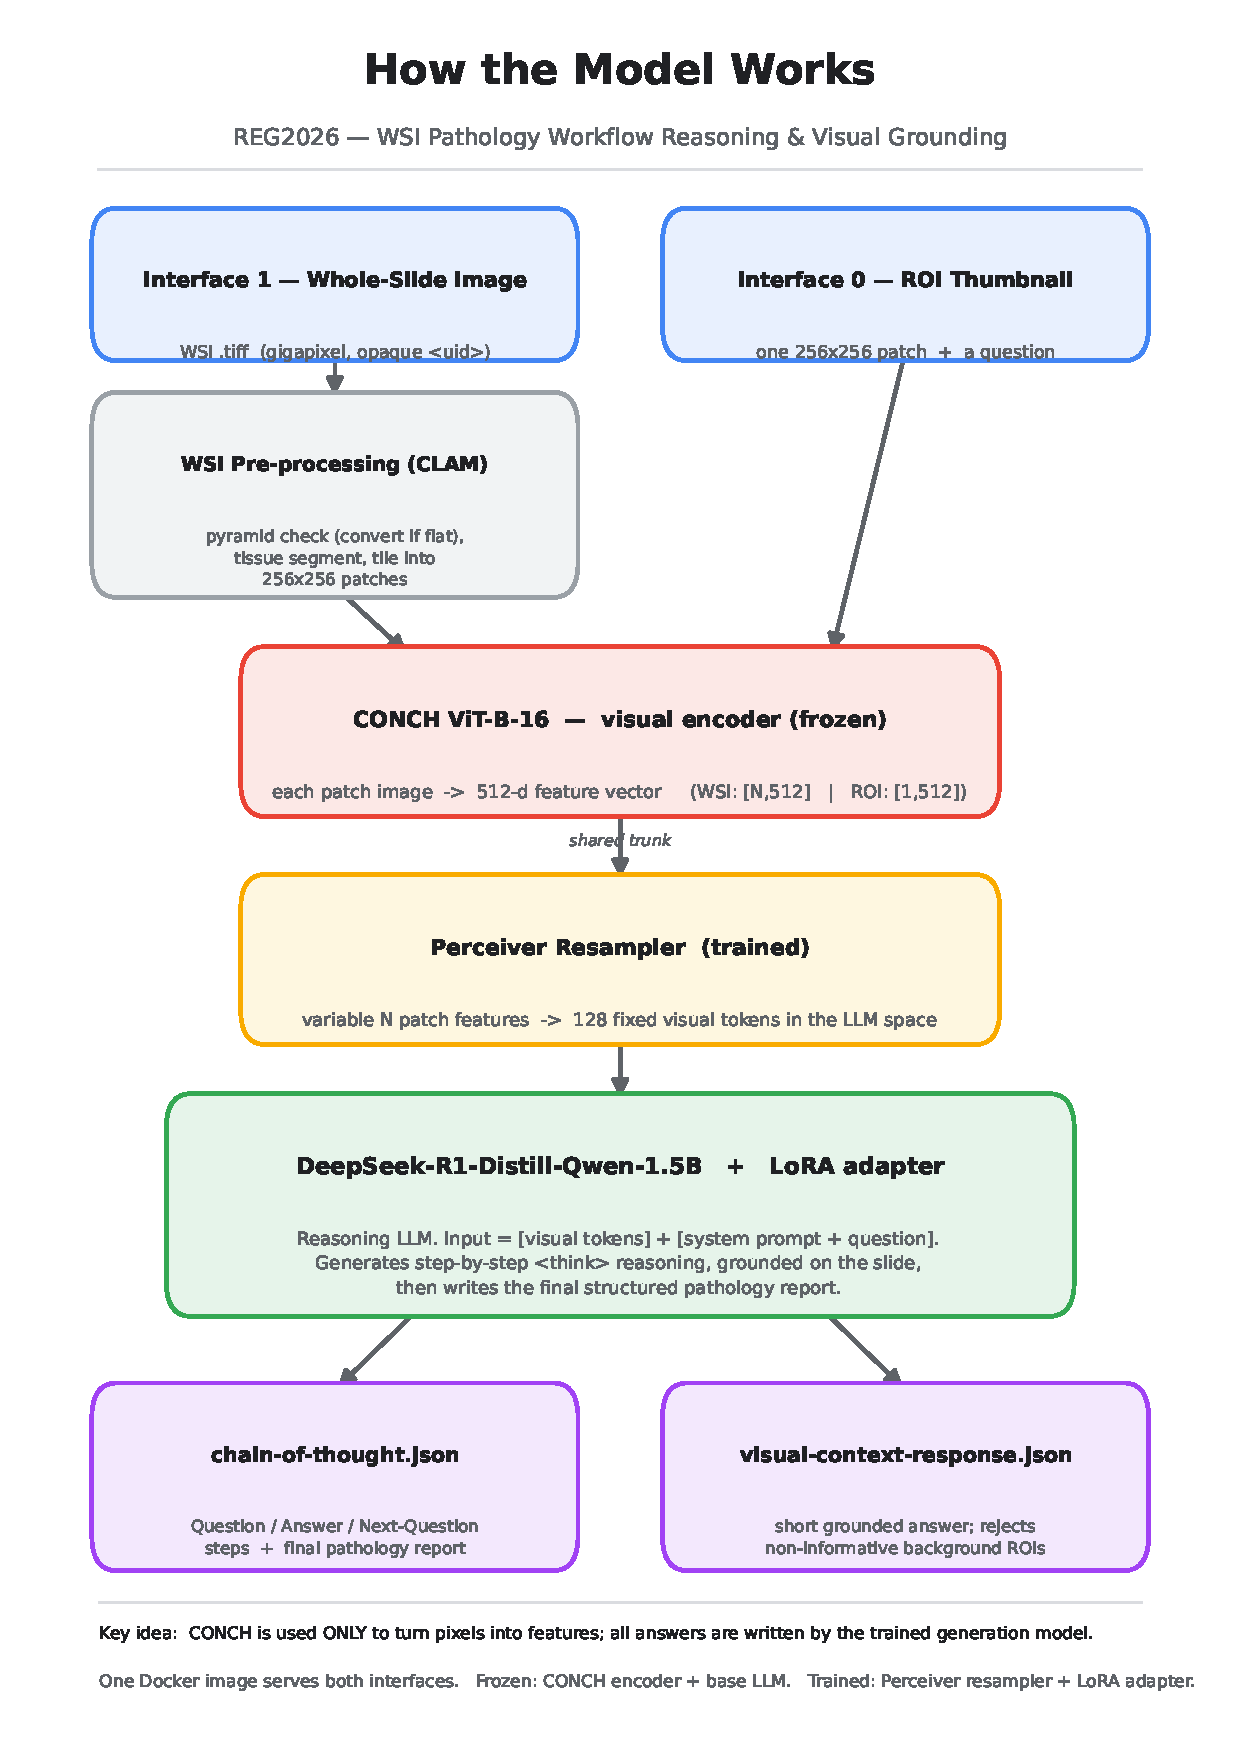
\includegraphics[width=\linewidth]{model_overview.pdf}
\caption{End-to-end architecture. CONCH (ViT-B/16) encodes tissue patches into a
variable-length bag $\Xbag\in\R^{N\times512}$. A Perceiver resampler with $K{=}128$
learned latent queries cross-attends the bag at every layer and emits a fixed set
of visual tokens $\Vvis$. These are concatenated with the embedded system/user
chat prompt and fed to a LoRA-adapted DeepSeek-R1-Distill-Qwen decoder, which
generates the \code{<think>} reasoning chain followed by the structured pathology
report. The cross-entropy loss is applied only to the assistant tokens (shaded).}
\label{fig:arch}
\end{figure}

\subsection{Perceiver resampler}
\label{sec:resampler}
The resampler is the module that reconciles an orderless, arbitrarily large bag
with a decoder that expects a small, fixed number of tokens. An input projection
$W_{\text{in}}\in\R^{d_v\times d}$ lifts the normalized bag to the decoder width,
$\mathbf{H}=\hat{\Xbag}\,W_{\text{in}}\in\R^{N\times d}$. A set of $K$ learned
latent queries $\Zlat^{0}\in\R^{K\times d}$, shared across all slides, is refined
over $L{=}3$ pre-norm blocks. Writing multi-head attention as
\begin{equation}
\Attn(\mathbf{q},\mathbf{k},\mathbf{v})=
\softmax\!\Big(\tfrac{\mathbf{q}\mathbf{k}^\top}{\sqrt{d_h}}\Big)\mathbf{v},
\qquad
\MHA(\cdot)=\big[\Attn_1;\dots;\Attn_h\big]W_O,
\end{equation}
with $h{=}8$ heads of width $d_h{=}d/h$~\cite{vaswani2017attention}, block $\ell$
applies latent-to-patch cross-attention, latent self-attention, and a
feed-forward network, each residual:
\begin{align}
\Zlat'_{\ell} &= \Zlat_{\ell-1}+\MHA\big(\LN(\Zlat_{\ell-1}),\,\mathbf{H},\,\mathbf{H}\big),
\label{eq:cross}\\
\Zlat''_{\ell} &= \Zlat'_{\ell}+\MHA\big(\LN(\Zlat'_{\ell}),\,\LN(\Zlat'_{\ell}),\,\LN(\Zlat'_{\ell})\big),
\label{eq:self}\\
\Zlat_{\ell} &= \Zlat''_{\ell}+\FFN\big(\LN(\Zlat''_{\ell})\big).
\label{eq:ffn}
\end{align}
The design is deliberate. Cross-attention~\eqref{eq:cross} keys and values are the
\emph{patches themselves}, so at every layer the latents re-query the raw bag
rather than a single pooled summary---this is what preserves the distributed,
region-indexed evidence that pooling-based MIL discards. Self-attention~\eqref{eq:self}
lets the $K$ latents specialize and de-duplicate, allocating queries across
distinct morphological regions. The output
$\Vvis\coloneqq\Zlat_{L}\in\R^{K\times d}$ is constant in size for any $N$, so a
slide with $10^2$ or $10^5$ patches presents the decoder with the same $128$
tokens. The resampler runs in the decoder's bf16 compute dtype to bound the
activation footprint of attending $K$ queries over thousands of patches.

\subsection{Multimodal fusion and prompt assembly}
\label{sec:fusion}
Fusion is performed in the decoder's input-embedding space rather than through a
separate cross-attention stack, which keeps the decoder architecturally
unmodified and lets LoRA adapt it in place. We build the chat prompt from a
pathologist \emph{system} message and a \emph{user} instruction using the
decoder's chat template, and embed its token ids with the decoder embedding matrix
$E$ to obtain $\Prompt = E(\text{prompt})\in\R^{|P|\times d}$. The visual tokens
are prepended, forming the fused input sequence
\begin{equation}
\mathbf{U} = \big[\,\Vvis\,;\,\Prompt\,\big]\in\R^{(K+|P|)\times d},
\end{equation}
which is passed to the decoder as \code{inputs\_embeds}. Because the visual and
text streams share one embedding space and one causal self-attention stack, every
generated token attends to all $K$ visual tokens at every layer, so grounding is
available throughout decoding rather than only at a bottleneck. The system prompt
fixes the output schema and instructs the decoder to reuse the canonical workflow
question strings verbatim, which is essential for the exact-match structure that
Metric~A rewards.

\subsection{Visually-conditioned reasoning decoder}
\label{sec:decoder}
The decoder is DeepSeek-R1-Distill-Qwen-1.5B~\cite{deepseek2025r1}, a decoder
distilled to emit an explicit reasoning span before its answer. We preserve this
behavior and adapt it with LoRA~\cite{hu2022lora}: for each adapted projection
$W_0\in\R^{d_{\text{out}}\times d_{\text{in}}}$ the forward map becomes
\begin{equation}
W_0\mathbf{u}\;\longmapsto\;W_0\mathbf{u}+\tfrac{\alpha}{r}\,BA\,\mathbf{u},
\qquad A\in\R^{r\times d_{\text{in}}},\;B\in\R^{d_{\text{out}}\times r},
\end{equation}
with rank $r{=}16$, scaling $\alpha{=}32$, and dropout $0.05$, applied to all
attention and MLP projections (\code{q/k/v/o\_proj}, \code{gate/up/down\_proj});
$B$ is zero-initialized so training begins at the pretrained function. Only
$\{A,B\}$ and the resampler are trainable---roughly $0.6\%$ of the decoder's
parameters---so the reasoning prior is retained rather than overwritten by a small
pathology corpus. The R1 chat template forces an opening \code{<think>} token,
which we also supply in the target; the forced token is stripped from the target
to avoid duplication. The same architecture supports QLoRA (NF4 4-bit
base~\cite{dettmers2023qlora}) and \code{device\_map} sharding for $7$B/$14$B
decoders, but the deployed configuration is the bf16 $1.5$B model
(Table~\ref{tab:hparams}).

\subsection{Target serialization}
\label{sec:format}
We serialize the diagnostic workflow into the reasoning decoder's native format.
The ordered steps are rendered as numbered \code{Question:\,/\,Answer:\,/\,Next
Question:} lines and wrapped, together with the report, into the R1 layout
\begin{center}
\code{<think>}\,\emph{reasoning}\,\code{</think>}\ \ \ \code{Pathology Report:}\,\emph{report}.
\end{center}
This is precisely the layout the decoder was distilled to produce, so generation
stays on the decoder's reasoning manifold rather than fighting it: the model
writes its chain of thought inside \code{<think>} tags and then commits to the
report after the marker. The format is line-oriented and unambiguous, which also
lets the generated string be read back into its constituent steps without any
post-processing. When the serialized target exceeds the $2048$-token budget,
truncation removes tokens from the \emph{reasoning} head while preserving the
entire final report, since the report is the primary diagnostic deliverable and
must be emitted in full, whereas an over-length reasoning tail can be shortened
with little loss of content.

\subsection{Training objective}
\label{sec:objective}
Each training sequence is $\mathbf{U}\;\Vert\;E(y)$, the fused input followed by
the embedded target tokens $y=(y_1,\dots,y_M)$. We minimize the negative
log-likelihood of the target under teacher forcing, but supervise \emph{only} the
assistant span: labels are set to the ignore index over the visual and prompt
positions, so the loss is
\begin{equation}
\label{eq:loss}
\mathcal{L}(\theta)= -\sum_{m=1}^{M}\mathbf{1}\!\left[m\in\mathcal{A}\right]\,
\log p_\theta\!\left(y_m \mid y_{<m},\,\Vvis,\,\Prompt\right),
\end{equation}
where $\mathcal{A}$ indexes the assistant (reasoning-plus-report) tokens and
$\theta$ collects the resampler and LoRA parameters. Masking the prompt and visual
spans prevents the model from wasting capacity re-predicting its own inputs and
concentrates the gradient on the reasoning steps and the report that constitute
the diagnostic output. We optimize~\eqref{eq:loss} with
AdamW (learning rate $2\times10^{-5}$, gradient clipping at $1.0$) for $3$ epochs
at effective batch size $32$ (per-device batch $1$, gradient accumulation $16$,
$2$ GPUs under DistributedDataParallel). Gradient checkpointing in DDP
\emph{static-graph} mode bounds activation memory for the long ($\approx\!2.7$k-token)
sequences: checkpointing reruns the forward pass during the backward pass, and
static-graph mode reconciles this with the gradient reducer. After every epoch the
model is generated-and-scored on a held-out subset with the full Metric~A
implementation, and a checkpoint (LoRA adapter, resampler, tokenizer, config) is
saved. Hyperparameters are summarized in Table~\ref{tab:hparams}.

\begin{table}[t]
\centering
\caption{Deployed model and training configuration.}
\label{tab:hparams}
\begin{tabular}{ll}
\toprule
\textbf{Component} & \textbf{Setting}\\
\midrule
Patch encoder            & CONCH ViT-B/16, frozen, $512$-d output\\
Resampler                & Perceiver, $K{=}128$ tokens, depth $3$, $8$ heads\\
Decoder (LLM)            & DeepSeek-R1-Distill-Qwen-1.5B, bf16\\
Adaptation               & LoRA $r{=}16$, $\alpha{=}32$, dropout $0.05$, all attn+MLP\\
Visual feature dim       & $512$ \quad(variant: $1024$-d, 7B decoder, $256$ tokens)\\
Max prompt / target len  & $512$ / $2048$ tokens\\
Optimizer                & AdamW, lr $2\times10^{-5}$, grad-clip $1.0$\\
Schedule                 & $3$ epochs; batch $1\times$ accum $16\times$ $2$ GPUs (eff.\ $32$)\\
Parallelism              & DDP + gradient checkpointing + static graph\\
Precision                & bf16 (LoRA + resampler trainable; base frozen)\\
\bottomrule
\end{tabular}
\end{table}

\subsection{Inference}
\label{sec:inference}
At test time the decoder receives only the fused input $\mathbf{U}=[\Vvis;\Prompt]$
and decodes greedily ($\arg\max$ at each step) for up to $1800$ new tokens.
Because \code{inputs\_embeds} is supplied, a decoder-only model returns only the
newly generated tokens, so no slicing of the prompt is required; the generated
string is passed directly through the Metric~A parser. The same generator, given a
one-patch ``slide,'' answers ROI questions for Visual Grounding
(Section~\ref{sec:grounding}).

\subsection{Complexity}
\label{sec:complexity}
The design isolates all slide-size dependence in the resampler. Cross-attention
in each of the $L$ blocks costs $O(KNd)$ and self-attention/FFN cost $O(K^2d)$,
giving a resampler cost of $O\!\big(L(KN+K^2)d\big)$ that is \emph{linear} in the
patch count $N$. The decoder then operates on a sequence of length
$K+|P|+|y|$ that is \emph{independent} of $N$, so the entire language stack---by
far the most expensive component---has cost invariant to slide size. This is the
property that makes gigapixel inference tractable: doubling the number of patches
at most doubles a single linear-in-$N$ cross-attention, and never enlarges the
decoder's context. The patch cap deployed for latency (Section~\ref{sec:deploy})
bounds even this term without changing the $K{=}128$ tokens the decoder sees.

\subsection{Visual Grounding pipeline}
\label{sec:grounding}
Metric~B is served by the same trained model through a self-contained two-stage
pipeline, kept separate from the training code (it imports only
\code{load\_generator} and \code{load\_wsi\_features}). \emph{Stage 1} encodes
each $256{\times}256$ ROI with a vendored, pure-Python CONCH into the identical
$[1,512]$ format as a WSI patch, exploiting the encoder- and normalization-sharing
of Section~\ref{sec:input} so that an ROI is numerically a one-patch slide.
\emph{Stage 2} queries the trained reasoning model per ROI and records each answer
together with its tissue/background label, its original/perturbed variant, and the
B3 pairing metadata required to compute B1/B2/B3. An optional ROI-focused system
prompt biases the model toward brief, grounded answers and explicit abstention on
non-informative regions, directly targeting the behavior B1 and B3 reward. The
released ROI set contains $18$ regions ($12$ tissue, $6$ background; $12$ original,
$6$ perturbed). Stage-1 features and Stage-2 answers run end-to-end; the final
B1/B2/B3 aggregation requires an external pathology judge LLM and is the remaining
step (Section~\ref{sec:limits}).

%==============================================================================
\section{Experiments}
\label{sec:results}
%==============================================================================
\subsection{Implementation details}
Patch extraction runs under PyTorch~2.1 with timm and the CONCH weights;
checkpoint loading and generation use a newer PyTorch~2.8 / Transformers~4.57 /
PEFT~0.17 stack so the LoRA adapter (serialized with a recent PEFT) deserializes.
Generation is greedy (\code{do\_sample=False}) with up to $1800$ new tokens.
Metric~A uses PubMedBERT embeddings for MESS and the report cosine. All test
numbers are computed on the $223$-case hold-out of Table~\ref{tab:data}.

\subsection{Main results}
Table~\ref{tab:test} reports the four Metric~A components and the combined score.
The model attains a Workflow Reasoning Score of $\mathbf{0.721}$. The profile of
the four terms is internally coherent and interpretable. Edge-F1 is the strongest
component at $0.807$, indicating that the predicted reasoning steps overlap the
reference steps well and that the model reliably reproduces the canonical
question/answer transitions. Exact-match BPV ($0.565$) is, as expected, the
hardest term, since it credits a case only when \emph{every} transition is
recovered; the gap between Edge-F1 and BPV is precisely the population of cases in
which most---but not all---transitions are correct. MESS ($0.756$) shows that answers on recovered edges
are semantically close to the references, confirming the model reasons about
content rather than merely reproducing question strings. The Final Report Score
($0.655$), the most heavily weighted term, indicates clinically plausible reports
and, given its $0.40$ weight, is the single largest contributor to the aggregate.

\begin{table}[t]
\centering
\caption{Workflow Reasoning results on the $223$-case held-out test set. All
components lie in $[0,1]$; higher is better. Parenthetical values are the
Metric~A weights of Eq.~\eqref{eq:wrs}.}
\label{tab:test}
\begin{tabular}{lc}
\toprule
\textbf{Component (weight)} & \textbf{Score}\\
\midrule
Binary Path Validity \;($0.05$) & $0.565$\\
Edge-F1 \;($0.30$)              & $0.807$\\
MESS \;($0.25$)                 & $0.756$\\
Final Report Score \;($0.40$)   & $0.655$\\
\midrule
\textbf{Workflow Reasoning Score} & $\mathbf{0.721}$\\
\bottomrule
\end{tabular}
\end{table}

\subsection{Report-generation quality}
\label{sec:reportgen}
The Final Report Score in Table~\ref{tab:test} is a challenge-specific composite;
to place the generated reports on a footing comparable to the report-generation
literature, Table~\ref{tab:reportgen} reports standard surface- and
embedding-level metrics computed on the same $223$ cases, comparing the
\emph{extracted} pathology report against its reference. BLEU-$n$ and
GLEU~\cite{wu2016gnmt} are corpus-level (NLTK, method-1 smoothing), ROUGE-L is the
mean per-report stemmed F1, and BERTScore~\cite{zhang2020bertscore} is the mean
token-level F1 under a RoBERTa-large backbone (no baseline rescaling, so absolute
values are high, as is typical for this metric).

The results are consistent with the qualitative picture from FRS. Lexical overlap
is high at the unigram level (BLEU-1 $0.725$, ROUGE-L $0.736$) and decays
gracefully with $n$-gram order (BLEU-2/3/4 $=0.676/0.634/0.596$), the signature of
reports that reproduce the correct clinical vocabulary and short phrases while
diverging on exact long-span wording. GLEU ($0.540$), a recall-sensitive
corpus metric, tracks BLEU-4 closely. The embedding-level BERTScore F1 ($0.959$)
confirms that generated and reference reports are close in a contextual semantic
space, not merely in surface tokens. We stress that the BLEU-4 reported here is a
corpus-level, smoothed score on the report text and is \emph{not} the same
quantity as the BLEU-4 sub-term folded into FRS (Section~\ref{sec:metrics}), which
uses a different tokenizer and enters only at weight $0.15$; the two numbers
should not be compared directly.

\begin{table}[t]
\centering
\caption{Report-generation quality on the $223$-case test set, comparing the
generated pathology report against the reference. BLEU-$n$ and GLEU are
corpus-level with method-1 smoothing; ROUGE-L is the mean per-report stemmed F1;
BERTScore is the mean token-level F1 (RoBERTa-large, no baseline rescaling). All
scores lie in $[0,1]$; higher is better.}
\label{tab:reportgen}
\begin{tabular}{lc}
\toprule
\textbf{Metric} & \textbf{Score}\\
\midrule
BLEU-1          & $0.725$\\
BLEU-2          & $0.676$\\
BLEU-3          & $0.634$\\
BLEU-4          & $0.596$\\
ROUGE-L (F1)    & $0.736$\\
GLEU            & $0.540$\\
BERTScore (F1)  & $0.959$\\
\bottomrule
\end{tabular}
\end{table}

\subsection{Training dynamics and component ablation over epochs}
Because every component is scored after each epoch, the training trajectory
doubles as a controlled study of \emph{which} capabilities the resampler and
adapters acquire, and in what order. Table~\ref{tab:epochs} tracks the in-training
validation score on a random $10$-case subset; these values are optimistic and
noisier than the full test set due to the small resampled subset, and we read them
for trends rather than absolute levels. Every component improves monotonically
across the three epochs, and the combined score rises from $0.543$ to $0.834$.
The most informative signal is the differential rate of improvement: BPV more than
doubles ($0.300\!\to\!0.700$) while Edge-F1 is already high after epoch~1
($0.666$). This ordering---partial structural overlap emerging early, exact
match consolidating late---is what one expects if the model first learns the
canonical question vocabulary and local transitions and only later stitches them
into globally consistent chains.\footnote{Here ``transition'' refers to the
metric's edge between a question and its next question; it is a property of how
Metric~A scores the sequence, not a structure the model predicts explicitly.}
FRS improves in lockstep ($0.453\!\to\!0.775$),
indicating that reasoning structure and report quality are learned jointly rather
than traded off, consistent with the shared assistant-token objective
of~\eqref{eq:loss}.

\begin{table}[t]
\centering
\caption{In-training validation (random $10$-case subset) by epoch. Values are
optimistic and noisier than Table~\ref{tab:test} due to the small resampled
subset; the trends, not the absolute levels, are the object of study.}
\label{tab:epochs}
\begin{tabular}{lccc}
\toprule
\textbf{Component} & \textbf{Epoch 1} & \textbf{Epoch 2} & \textbf{Epoch 3}\\
\midrule
Binary Path Validity      & $0.300$ & $0.500$ & $0.700$\\
Edge-F1                   & $0.666$ & $0.737$ & $0.889$\\
MESS                      & $0.590$ & $0.693$ & $0.889$\\
Final Report Score        & $0.453$ & $0.563$ & $0.775$\\
\midrule
\textbf{Workflow Reasoning Score} & $0.543$ & $0.645$ & $\mathbf{0.834}$\\
\bottomrule
\end{tabular}
\end{table}

\subsection{Qualitative analysis of Visual Grounding}
The ROI extraction and question-answering stages run end-to-end on the released
$18$-ROI set, producing per-ROI answers with the metadata required for B1/B2/B3.
Qualitatively, with the ROI-focused system prompt the model abstains on background
regions (\eg ``this region is background / not assessable'') while giving
content-bearing answers on tissue ROIs---the behavior B1 (background rejection)
and B3 (tissue--background separation) reward. This asymmetry is direct evidence
that the model conditions on the visual token rather than emitting a
context-independent template, since the prompt is held fixed across ROIs and only
the single visual token changes. Quantitative B1/B2/B3 values require the external
judge model and are deferred (Section~\ref{sec:limits}); we do not claim them
here.

\subsection{Computational efficiency}
The efficiency of the system follows from two decisions analyzed above. First, the
resampler makes decoder cost independent of slide size
(Section~\ref{sec:complexity}), so the language stack processes the same
$K{+}|P|{+}|y|$ tokens whether a slide has $10^2$ or $10^5$ patches. Second,
parameter-efficient adaptation trains only $\sim\!0.6\%$ of the decoder plus the
resampler, which is what permits the effective-batch-$32$ regime of
Table~\ref{tab:hparams} on two consumer GPUs. At deployment, merging the LoRA
adapter into the base weights removes the per-token low-rank matmuls at no change
to outputs, and a patch cap bounds the sole linear-in-$N$ term
(Section~\ref{sec:deploy}).

\subsection{Error analysis}
The metric decomposition localizes the model's residual errors. The dominant
signed gap is between Edge-F1 ($0.807$) and BPV ($0.565$): most failures are not
wholesale hallucinations of the reasoning chain but single missing or spurious
transitions that forfeit the all-or-nothing BPV credit while leaving Edge-F1
largely intact. Because BPV carries only weight $0.05$, these near-misses cost
little in
aggregate, but they identify long or atypical chains---where one mis-predicted
transition breaks exact match---as the structural failure mode. On content,
MESS ($0.756$) exceeds FRS ($0.655$), indicating that short intermediate answers
are recovered more reliably than the long free-text report; report generation,
not edge prediction, is therefore the accuracy bottleneck, in agreement with the
weighting analysis below.

\subsection{Limitations}
The evaluation has three notable limits. Metric~B is not yet scored end-to-end:
ROI features and answers are produced, but B1/B2/B3 require a pathology judge LLM
that is not integrated. The per-epoch numbers of Table~\ref{tab:epochs} come from
a $10$-case subset and are optimistic relative to the $223$-case test set.
Finally, all results use greedy decoding; sampling-based decoding and larger
validation splits are unexamined. These points are expanded in
Section~\ref{sec:limits}.

%==============================================================================
\section{Containerized Deployment}
\label{sec:deploy}
%==============================================================================
The challenge executes submissions as an offline container, with weights mounted
separately and no network access. A single image serves both interfaces.
\textbf{Interface~0} maps an ROI \code{.jpeg} to one answer string
(CONCH~$\to[1,512]\to$ generation), and \textbf{Interface~1} maps a WSI
\code{.tiff} to a chain-of-thought array (pyramid conversion if needed $\to$ CLAM
segmentation and patching $\to$ CONCH $[N,512]\to$ generation $\to$ schema
parser). Each handler wraps inference in a guarded fallback so that no single case
can leave a missing output.

A first online run completed most cases but halted on a single outlier slide that
exceeded the per-case time limit. We added four latency safeguards, each chosen to
leave accuracy on normal cases unchanged. (1)~\emph{Patch cap}: if a slide yields
more than $\mathrm{REG\_MAX\_PATCHES}$ ($12{,}000$) patches, coordinates are
uniformly (evenly-strided) subsampled before encoding; because the resampler
compresses to $128$ tokens regardless (Section~\ref{sec:complexity}), coverage is
preserved and normal slides are untouched. (2)~\emph{LoRA merge}: the adapter is
merged into the base weights at load time (\code{merge\_and\_unload}), making
decoding mathematically identical while dropping the per-token low-rank matmuls.
(3)~\emph{Throughput}: larger CONCH inference batches and more data-loader workers
(pure I/O, no effect on outputs). (4)~\emph{Generation budget}: a
\code{MaxTimeCriteria} ($180$\,s default) returns truncated-but-parseable text
instead of allowing a runaway decode to kill the submission. Because the merge
happens at load time, the weights are unchanged and only the container image is
re-uploaded.

%==============================================================================
\section{Discussion}
\label{sec:discussion}
%==============================================================================
Three design choices explain the measured behavior. \emph{Native-format
supervision} (Section~\ref{sec:format}) serializes the workflow in the decoder's
own reasoning layout and restricts the loss to assistant tokens~\eqref{eq:loss},
so training concentrates on the stepwise reasoning and the report; this is the
mechanism behind the strong Edge-F1 and the steep BPV gains across epochs. \emph{Constant-size visual grounding}
(Sections~\ref{sec:resampler} and~\ref{sec:complexity}) decouples decoder cost
from slide size, which is what makes both training memory and worst-case latency
manageable and, at deployment, what lets a patch cap bound runtime without
altering the $128$ tokens the decoder consumes. \emph{Parameter efficiency}
(Section~\ref{sec:decoder}) trains only the adapters and resampler over a frozen
$1.5$B reasoner, retaining its native reasoning ability on modest hardware.

The held-out profile also indicates where the next gains lie. Report quality is
the binding constraint: at weight $0.40$ in~\eqref{eq:wrs}, each $0.01$ of FRS is
worth as much as $0.08$ of BPV, so the FRS of $0.655$---the lowest-scoring
high-weight term---is the highest-value target. The error analysis reinforces
this: intermediate answers (MESS $0.756$) are recovered more reliably than the
report (FRS $0.655$), so report-focused decoding, retrieval of canonical report
templates, or light reinforcement against FRS are the most promising directions.

%==============================================================================
\section{Limitations and Future Work}
\label{sec:limits}
%==============================================================================
\emph{Metric~B is not yet scored end-to-end.} ROI features and answers are
produced, but B1/B2/B3 require a pathology judge LLM that is not yet integrated;
wiring in a local judge and reporting Visual Grounding numbers is the immediate
next step. \emph{Report quality is the binding constraint}, and given its $0.40$
weight, report-focused decoding, template retrieval, or reinforcement against the
Final Report Score are the highest-value improvements. \emph{Decoder scale} is
capped for latency and memory: the codebase already supports $7$B/$14$B decoders
via QLoRA and \code{device\_map}, and scaling is expected to raise MESS and report
fidelity most. Finally, \emph{decoding and validation} are conservative: results
use greedy generation, and the per-epoch numbers come from a $10$-case subset that
is optimistic relative to the $223$-case test set, so sampling-based decoding and
larger validation splits deserve study.

%==============================================================================
\section{Conclusion}
%==============================================================================
We presented a compact, end-to-end system for diagnostic workflow reasoning and
pathology report generation from whole-slide images. Casting the task as
visually-conditioned sequence generation, we compress a frozen CONCH patch bag
into a constant $128$ visual tokens with a Perceiver resampler and let a
LoRA-adapted DeepSeek-R1 reasoning decoder generate the entire diagnostic chain in
its native reasoning format. Trained only on low-rank adapters and the resampler,
the model reaches a Workflow Reasoning Score of $0.721$ on a $223$-case hold-out,
recovering the reasoning structure well (Edge-F1 $0.807$). We additionally
contribute a CONCH-based ROI grounding pipeline for the Visual Grounding metric and
a fully offline, latency-hardened container serving both challenge interfaces. The
system demonstrates that faithful and auditable pathology reasoning over gigapixel
slides is achievable with a parameter-efficient multimodal model on modest
hardware.

%==============================================================================
\section*{Reproducibility and Data Availability}
%==============================================================================
The model, training, and evaluation code---feature extraction, Perceiver
resampler, reasoning decoder, the Metric~A reimplementation, the ROI grounding
pipeline, and the deployment container---are organized in the project repository.
Training uses the REG2026 chain-of-thought corpus; CONCH weights follow the CONCH
release. Each checkpoint stores the LoRA adapter, resampler weights, tokenizer, and
configuration for exact reload.

%==============================================================================
\begin{thebibliography}{99}
\setlength{\itemsep}{2pt}

\bibitem{lu2024conch}
M.~Y. Lu, B. Chen, D.~F.~K. Williamson, \emph{et al.},
``A visual--language foundation model for computational pathology,''
\emph{Nature Medicine}, vol.~30, pp.~863--874, 2024.

\bibitem{lu2021clam}
M.~Y. Lu, D.~F.~K. Williamson, T.~Y. Chen, \emph{et al.},
``Data-efficient and weakly supervised computational pathology on whole-slide
images,'' \emph{Nature Biomedical Engineering}, vol.~5, pp.~555--570, 2021.

\bibitem{chen2024uni}
R.~J. Chen, T. Ding, M.~Y. Lu, \emph{et al.},
``Towards a general-purpose foundation model for computational pathology,''
\emph{Nature Medicine}, vol.~30, pp.~850--862, 2024.

\bibitem{ilse2018attention}
M. Ilse, J.~M. Tomczak, and M. Welling,
``Attention-based deep multiple instance learning,''
in \emph{Proc. ICML}, 2018, pp.~2127--2136.

\bibitem{deepseek2025r1}
DeepSeek-AI,
``DeepSeek-R1: Incentivizing reasoning capability in LLMs via reinforcement
learning,'' arXiv:2501.12948, 2025.

\bibitem{yang2024qwen2}
A. Yang, B. Yang, B. Hui, \emph{et al.},
``Qwen2 technical report,'' arXiv:2407.10671, 2024.

\bibitem{hu2022lora}
E.~J. Hu, Y. Shen, P. Wallis, \emph{et al.},
``LoRA: Low-rank adaptation of large language models,''
in \emph{Proc. ICLR}, 2022.

\bibitem{dettmers2023qlora}
T. Dettmers, A. Pagnoni, A. Holtzman, and L. Zettlemoyer,
``QLoRA: Efficient finetuning of quantized LLMs,''
in \emph{Proc. NeurIPS}, 2023.

\bibitem{alayrac2022flamingo}
J.-B. Alayrac, J. Donahue, P. Luc, \emph{et al.},
``Flamingo: A visual language model for few-shot learning,''
in \emph{Proc. NeurIPS}, 2022.

\bibitem{jaegle2021perceiver}
A. Jaegle, F. Gimeno, A. Brock, \emph{et al.},
``Perceiver: General perception with iterative attention,''
in \emph{Proc. ICML}, 2021, pp.~4651--4664.

\bibitem{li2023blip2}
J. Li, D. Li, S. Savarese, and S. Hoi,
``BLIP-2: Bootstrapping language-image pre-training with frozen image encoders
and large language models,'' in \emph{Proc. ICML}, 2023.

\bibitem{liu2023llava}
H. Liu, C. Li, Q. Wu, and Y.~J. Lee,
``Visual instruction tuning,'' in \emph{Proc. NeurIPS}, 2023.

\bibitem{dosovitskiy2021vit}
A. Dosovitskiy, L. Beyer, A. Kolesnikov, \emph{et al.},
``An image is worth $16\times16$ words: Transformers for image recognition at
scale,'' in \emph{Proc. ICLR}, 2021.

\bibitem{vaswani2017attention}
A. Vaswani, N. Shazeer, N. Parmar, \emph{et al.},
``Attention is all you need,'' in \emph{Proc. NeurIPS}, 2017.

\bibitem{gu2021pubmedbert}
Y. Gu, R. Tinn, H. Cheng, \emph{et al.},
``Domain-specific language model pretraining for biomedical natural language
processing,'' \emph{ACM Trans. Computing for Healthcare}, vol.~3, no.~1, 2021.

\bibitem{papineni2002bleu}
K. Papineni, S. Roukos, T. Ward, and W.-J. Zhu,
``BLEU: A method for automatic evaluation of machine translation,''
in \emph{Proc. ACL}, 2002, pp.~311--318.

\bibitem{lin2004rouge}
C.-Y. Lin,
``ROUGE: A package for automatic evaluation of summaries,''
in \emph{Text Summarization Branches Out}, ACL Workshop, 2004, pp.~74--81.

\bibitem{wu2016gnmt}
Y. Wu, M. Schuster, Z. Chen, \emph{et al.},
``Google's neural machine translation system: Bridging the gap between human and
machine translation,'' arXiv:1609.08144, 2016.

\bibitem{zhang2020bertscore}
T. Zhang, V. Kishore, F. Wu, K.~Q. Weinberger, and Y. Artzi,
``BERTScore: Evaluating text generation with BERT,''
in \emph{Proc. ICLR}, 2020.

\end{thebibliography}

\end{document}
